\documentclass[a4paper,12pt]{scrartcl} 

%\usepackage[latin1]{inputenc} 
%Apple \usepackage[applemac]{inputenc} 
\usepackage[utf8]{inputenc}
\usepackage[ngerman]{babel}
\usepackage[T1]{fontenc}

%Das Paket erzeugt ein anklickbares Verzeichnis in der PDF-Datei.
\usepackage[hyperfootnotes=false,colorlinks=true,linkcolor=black,urlcolor=black]{hyperref}

%Das Paket wird fr die anderthalb-zeiligen Zeilenabstand bentigt
\usepackage{setspace}

%Einrückung eines neuen Absatzes
\setlength{\parindent}{0em}

%Definition der Rnder
\usepackage[paper=a4paper,left=30mm,right=30mm,top=30mm,bottom=30mm]{geometry} 

\usepackage{amsfonts}
\usepackage{amsmath}
\usepackage{cancel}
\usepackage{graphicx}
\usepackage{mathcomp}
\usepackage{polynom}
\usepackage{hyperref}

%Abstand der Fußnoten
\deffootnote{1em}{1em}{\textsuperscript{\thefootnotemark\ }}

%Regeln, bis zu welcher Tiefe (section,subsection,subsubsection) Überschriften angezeigt werden sollen (Anzeige der Überschriften im Verzeichnis / Anzeige der Nummerierung)
\setcounter{tocdepth}{3}
\setcounter{secnumdepth}{3}

%-------------------
%Ende des Kopfbereiches
%-------------------


\begin{document}

%Beginn der Titelseite
\begin{titlepage}
\begin{small}
\vfill {AKAD\\ 
Bachelor of Science (Wirtschaftsinformatik) \\ 
Modulzusammenfassung}
\end{small}


\begin{center}
\begin{Large}
\vfill {\textsf{\textbf{
WIM04 \\
\vspace*{1cm} 
Formelsammlung
}}}
\end{Large}
\end{center}

\begin{small}
\vfill Daniel Falkner \\ Rotbach 529 \\  94078 Freyung \\  daniel.falkner@akad.de \\ 
\today
\end{small}

\end{titlepage}
%Ende der Titelseite


%Inhaltsverzeichnis (aktualisiert sich erst nach dem zweiten Setzen)
\tableofcontents
\thispagestyle{empty}

%Beginn einer neuen Seite
\clearpage

%Anderthalbzeiliger Zeilenabstand ab hier
\onehalfspacing

\pagestyle{plain}


\section{Folgen}
Eine Serie von Zahlen oder Größen \\
5, 10, 4, 1 \\
$(a_n) = a_1, a_2, a_3, .., a_n$
\subsection{arithmetische Folgen}
\begin{itemize}
\item $a_{n+1} = a_n + d$ 
\item 7, 11, 15, 19, 23, 27, ... 
\item $\mapsto d = 4$ 
\end{itemize}

\subsubsection{Bildungsgesetz}
$a_n = a_1 + d * (n - 1)$

\subsubsection{Grenzwerte}
Eine arithmetische Folge divergiert immer (wird beliebig groß), wenn $d \ne 0$

\subsection{geometrische Folgen}
\begin{itemize}
\item $a{n+1} = a_n * q$
\item 2, 6, 18, 54, 162, 486, ...
\item $\mapsto q = 3$
\end{itemize}

\subsubsection{Bildungsgesetz}
$a_n = a_1 * q^{n - 1} \Leftrightarrow q = \sqrt[n-1]{\cfrac{a_n}{a_1}}$

\subsubsection{Grenzwerte}
Das Verhalten einer geometrischen Folge $n \mapsto a_n$ für wachsendes n hängt vom Quotienten q ab
\begin{itemize}
\item Falls $|q| < 1$, streben die Flieder $a_n$ der Folge gegen 0. Grenzwert 0 (konvergiert gegen 0)
\item Falls $|q| > 1$, werden für $a_1 \ne 0$ die $|a_n|$ beliebig groß, die Folge divergiert
\end{itemize}

\newpage
\section{Reihen}
Aus einer Folge ergibt sich eine Reihe \\
$(s_n) = s_1, s_2, s_3, ..., s_n$ \\
$(s_n) = a_1 + a_2 + a_3 + ... + a_n = \sum\limits_{j=1}^n a_j$

\subsection{arithmetische Reihen}
\begin{itemize}
\item $(a_n) = 7, 11, 15, 19, ... \mapsto a_1 = 7, d = 4$ 
\item $(s_n) = 7, 18, 33, 52, ...$
\end{itemize}

\subsubsection{Bildungsgesetz}
$s_n = \cfrac{n}{2} * (a_1 + a_n) = \cfrac{n}{2} * (2a_1 + (n - 1)d)$

\subsubsection{Grenzwerte}
Eine notwendige, aber nicht hinreichende Bedingung für die Konvergenz einer unendlichen Reihe ($s_n$) ist  	$\lim_{n \to \infty} a_n = 0$. Die Folge ($a_n$) muss also eine so genannte Nullfolge sein. 

\subsection{geometrische Reihen}
\begin{itemize}
\item $(a_n) = 2, 6, 18, 54, ... \mapsto a_1 = 2, q = 3$ 
\item $(s_n) = 2, 8, 26, 80, ...$
\end{itemize}

\subsubsection{Bildungsgesetz}
$s_n = a_1 * \cfrac{q^n - 1}{q - 1}, q \ne 1$

\subsubsection{Grenzwerte}
Eine unendliche geometrische Reihe ($s_n$) mit $s_n = \sum\limits_{k=1}^n a_1 q^{k-1}$ konvergiert genau gegen den Grenzwert $S=\cfrac{a_1}{1-q}$ wenn $|q| < 1$ ist.

\newpage
\section{Vollständige Induktion}
Am Beispiel $ 2 + 4 + 6 ... 2 * n = n + n^2$

\begin{enumerate}
\item Zeigen das die Formeln für n = 1 gelten

\begin{itemize}
\item $s_1 = 2 * n = 2 * 1 = 2$
\item $s_1 = n + n^2 = 1 + 1^2 = 2$
\end{itemize}

\item Zeigen das die Formeln für n + 1 gelten
\begin{enumerate}
\item Induktionsannahme \textit{(zu beweisende Formel)} festhalten 
\begin{itemize}
\item $s_n = n + n^2$
\end{itemize}

\item Die zubeweisende Formel für $n + 1$ herleiten
\begin{itemize}
\item $s_{n+1} = (n+1) + (n+1)^2 = n^2 + 3n + 2$
\end{itemize}

\item Die Induktionsnahme + Ursprungsformel für $n + 1$ herleiten
\begin{itemize}
\item $s_{n+1} =  n + n^2 + 2 (n+1) = n^2 + 3n + 2$
\end{itemize}
\end{enumerate}
\end{enumerate}

\newpage
\section{Determinanten}
\subsection{Regel von Sarrus}
\subsubsection{Für 2 x 2}

$
\det(A) = 
\det \begin{pmatrix}
a & b \\ 
c & d 
\end{pmatrix} = ad - cb.
$

\subsubsection{Für 3 x 3}
$ \det(A) = \det
\begin{pmatrix}
  a & b & c \\
  d & e & f \\
  g & h & i
\end{pmatrix} = aei + bfg + cdh - ceg -afh -bdi
$

\newpage
\subsection{CRAMER'sche Regel}
\begin{figure}[ht]
	\centering
  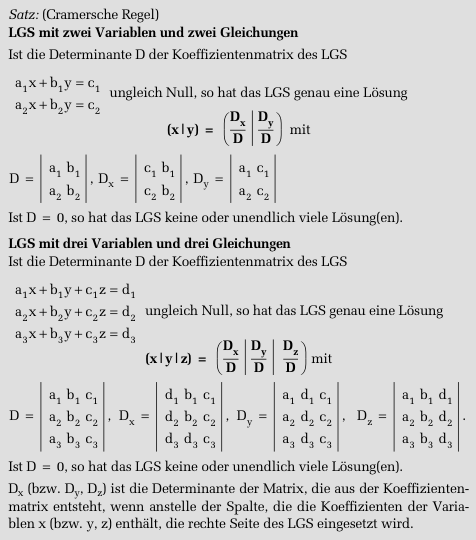
\includegraphics[width=1.0\textwidth]{wim01-zusammenfassung_cramersche_regel.png}
	\caption{AKAD WIM01 Mathematische Grundlagen, Lerneinheit 4, Seite 46}
	\label{fig01}
\end{figure}

\newpage
\section{Matrizen}
\subsection{Transponierte Matrix}
$A^T$ entsteht durch Vertauschen der Zeilen mit den Spalten von $A$\\

Beispiel: \\
$A_{(2,3)} = 
\begin{bmatrix}
 1 & 2 & 3\\
 -2 & 4 & -1 \\
\end{bmatrix}
A_{(3,2)}^T = 
\begin{bmatrix}
 1 & -2\\
 2 & 4\\
 3 & -1
\end{bmatrix}
$
\subsection{Addition}
\subsubsection{vom selben Typ}
die gleichstehenden Elemente addieren und zu einer neuen Matrix zusammenfassen

\subsection{Multiplikation}
\subsubsection{mit einer reellen Zahl (Skalar)}
alle Elemente der Matrix mit der Zahl multiplizeren

\subsubsection{zweier Matrizen}
Zwei Matrizen sind multiplikationsverträglich wenn die Spaltenanzahl von A mit der Zeilanzahl von B übereinstimmt. 
Eine Hilfe bietet das Falk-Schema \footnote{\url{http://de.wikipedia.org/wiki/Falksches_Schema}}

\subsubsection{spezielle Matrixprodukte}
\begin{itemize}
\item Zeilenvektor * Spaltenvektor = Skalar
\item Spaltenvektor * Zeilenvekor = Matrix
\end{itemize}


\subsection{Inverse}
\begin{itemize}
\item A vom Typ (n,n) ist regulär, d.h. $A^{-1}$ (Inverse Matrix) existiert. Dann ist die Matrixgleichung A * X = B eindeutig lösbar.
\item Eine quadratische Matrix A ist genau dann invertierbar, wenn ihre Determinate |A| ungleich Null ist
\end{itemize}

\subsubsection{Bestimmung der inversen Matrix}
\begin{itemize}
\item Die Inverse $A^{-1}$ lässt sich mit dem Gauß-Jordan-Verfahren \footnote{\url{http://de.wikipedia.org/wiki/Gau\%DF-Jordan-Algorithmus}} ermitteln
\end{itemize}

\subsubsection{mit Hilfe der Adjunktion}
\begin{enumerate}
\item Determinante bestimmen und prüfen ob  $A^{-1}$ existiert
\item Unterdeterminaten \footnote{\url{http://de.wikipedia.org/wiki/Minor_(Mathematik)}} bestimmen
\item Kofaktorenmatrix cof(A) anhand der Unterdeterminanten aufstellen. Bei ungeraden Indizies das Vorzeichen ändern
\item adjungierte Matrix aufstellen, indem die Kofaktorerenmatrix transponiert wird. \\ $adj(A) = [cof(A)]^T$
\item adjungierte Matrix mit dem Kehrwert der Determinate multiplizieren. \\ $\cfrac{1}{D} * adj(A)$
\end{enumerate}

\newpage
\section{Aussagenlogik}
\subsection{Verknüpfungen}

\subsubsection{Negation}
\begin{tabular}{l|c}
  p & $\neg$ p\\
  \hline
  w & f \\
  f & w \\
\end{tabular}

\subsubsection{Konjunktion (und)}
\begin{tabular}{lc|c}
  p & q & p $\land$ q\\
  \hline
  w & w & w \\
  w & f & f \\
  f & w & f \\
  f & f & f \\
\end{tabular}

\subsubsection{Disjunktion auch Adjunktion (oder)}
\begin{tabular}{lc|c}
  p & q & p $\vee$ q\\
  \hline
  w & w & w \\
  w & f & w \\
  f & w & w \\
  f & f & f \\
\end{tabular}
\\ 
\\ Die Verknüpfung durch das ausschließende oder (XOR) heißt Alternative oder Antivalenz \\

\begin{tabular}{lc|c}
  p & q & p XOR q\\
  \hline
  w & w & f \\
  w & f & w \\
  f & w & w \\
  f & f & f \\
\end{tabular}

\subsubsection{Subjunktion (wenn dann)}
\begin{tabular}{lc|c}
  p & q & p $\to$ q\\
  \hline
  w & w & w \\
  w & f & f \\
  f & w & w \\
  f & f & w \\
\end{tabular}
\\
\\ $\neg p \vee q$ \textit{ist gleich mit} $p \to q$

\subsubsection{Bijunktion (genau dann, wenn)}
\begin{tabular}{lc|c}
  p & q & p $\leftrightarrow$ q\\
  \hline
  w & w & w \\
  w & f & f \\
  f & w & f \\
  f & f & w \\
\end{tabular}
\\
\\ $(p \to q) \land (q \to p)$ \textit{ist gleich mit} $p \leftrightarrow q$
\\ $(p \land q) \vee (\neg p \land \neg q)$ \textit{ist gleich mit} $p \leftrightarrow q$

\subsubsection{Sonderformen}

\begin{itemize}
\item Ist die Aussage r für alle Belegungen p und q \textit{wahr}, so heißt r eine \textbf{Tautlogie}.
\item Ist die Aussage r für alle Belegungen von p und q \textit{falsch}, so heißt r eine  \textbf{Kontradiktion}.
\item Ist die Aussage r \textit{weder} eine Tautologie \textit{noch} eine Kontradiktion, so heißt r eine \textbf{Kontingenz} oder Neutralität.
\end{itemize}


\subsection{Gesetze}
\begin{tabular}{l|c|l}
  Verknüpfung $\land$ & Gesetze & Verknüpfung $\vee$\\
  \hline
  $p \land q \Leftrightarrow q \land p$ & Kommutativgesetz & $p \vee q \Leftrightarrow q \vee p$ \\
  $(p \land q) \land r \Leftrightarrow p \land (q \land r)$ & Assoziativgesetz & $(p \vee q) \vee r \Leftrightarrow p \vee (q \vee r)$ \\
  $p \land (q \vee r) \Leftrightarrow (p \land q) \vee (p \land r)$ & Distributivgesetz & $p \vee (q \land r) \Leftrightarrow (p \vee q) \land (p \vee r)$ \\
  $p \land p \Leftrightarrow p$ & Idempotenzgesetz & $p \vee p \Leftrightarrow p$ \\
  $p \land (p \vee q) \Leftrightarrow p$ & Absorptionsgesetz & $ p \vee (p \land q) \Leftrightarrow p$ \\  
  $p \land (w) \Leftrightarrow p$ & Neutrales Element & $p \vee (f) \Leftrightarrow p$ \\
   $p \land (f) \Leftrightarrow (f); p \land \neg p \Leftrightarrow (f)$ & Kontradiktion & \\
  & Trautologie &  $p \vee (w) \Leftrightarrow (w); p \vee \neg p \Leftrightarrow (w)$ \\
  $\neg (p \land q) \Leftrightarrow \neg p \vee \neg q$ & Regeln von de Morgen & $\neg (p \vee q) \Leftrightarrow \neg p \land \neg q$ \\
\end{tabular}


\subsection{Normalformen}

\subsubsection{Minterme}
Minterme sind genau diejenigen Konjunktionsterme, die den Wert 'w' nur einmal annehmen und mit dem Junktor $\land$ verknüpft sind.
\subsubsection{Maxterme}
Maxterme sind genau diejenigen Disjunktionsterme, die den Wert 'f' nur einmal annehmen und mit dem Junktor $\vee$ verknüpft sind.
\subsubsection{Kanonische disjunktive Normalform}
Ein Disjungat (Junktor $\vee$) paarweise verschiedener Minterme heißt Kanonische disjunktive Normalform \\ \\
\begin{tabular}{lcc|cc}
  A & B & C & x & \\
  \hline
  w & w & w & f & \\
  w & w & f & w & ergibt den Minterm $ A \land B \land \neg C$\\
  ... & ... & ... & ...\
\end{tabular}
\subsubsection{Kanonische konjunktive Normalform}
Ein Konjungat (Junktor $\land$) paarweiter verschiedener Maxterme heißt Kanonische konjunktive Normalform \\ \\
\begin{tabular}{lcc|cc}
  A & B & C & x & \\
  \hline
  w & w & w & f & ergibt den Maxterm $ \neg A \vee \neg B \vee \neg C$\\
  w & w & f & w & \\
  ... & ... & ... & ...\
\end{tabular}

\newpage
\section{Schaltalgebra}
\subsection{Gesetze}
\begin{tabular}{l|c|l}
  Verknüpfung $+$ & Gesetze & Verknüpfung $*$\\
  \hline
  $a + b = b + a$ & Kommutativgesetz & $a * b = b * a$ \\
  $a + (b * c) = (a + b)(a + c)$ & Distributivgesetz & $a * (b + c) = (a * b) + (a * c)$ \\
  $a + 0 = 0 + a = a$ & Neutrales Element & $a * 1 = 1 * a = a$ \\
  $a + \overline{a} = 1$ & Inverses Element & $a * \overline{a} = 0$\\
  \hline
  $(a + b) + c = a + (b + c)$ & Assoziativgesetz & $(a * b) * c = a * (b * c)$ \\
  $a + (a * b) = a$ & Absorptionsgesetz & $ a * (a + b) = a$ \\
  $a + 1 = 1$ & Trautologie & \\
   & Kontradiktion & $a * 0 = 0$ \\
  $a + a = a$ & Idempotenzgesetz & $a * a =a$ \\
  $\overline{a + b} = \overline{a} * \overline{b}$ & Regeln von de Morgen & $\overline{a * b} = \overline{a} + \overline{b}$ \\
\end{tabular}

\subsection{Normalformen}

\subsubsection{Minterme}
Minterme sind genau diejenigen vollständigen Produkte, die den Leitwert 1 genau dann annehmen, wenn jeder Faktor den Leitwert 1 annimmt.
\subsubsection{Maxterme}
Maxterme sind genau diejenigen vollständigen Summen, die den Leitwert 0 genau dann annehmen, wenn jeder Summand den Leitwert 0 annimmt.
\subsubsection{Kanonische disjunktive Normalform}
Die Summe der Minterme ergibt die Schaltfunktion in kanonischer disjunktiver Normalform \\ \\
\begin{tabular}{lcc|cc}
  a & b& c & f & \\
  \hline
  1 & 1 & 1 & 0 & \\
  1 & 1 & 0 & 1 & ergibt den Minterm $a * b * \overline{c}$\\
  ... & ... & ... & ...\
\end{tabular}
\subsubsection{Kanonische konjunktive Normalform}
Das Produkt der Maxterme ergibt die Schaltfunktion in kanonischer konjunktiver Normalform
 \\ \\
\begin{tabular}{lcc|cc}
  A & B & C & x & \\
  \hline
  1 & 1 & 1 & 0 & ergibt den Maxterm $\overline{a} + \overline{b} + \overline{c}$\\
  1 & 1 & 0 & 1 & \\
  ... & ... & ... & ...\
\end{tabular}

\newpage

\subsection{Logikgatter}
\subsubsection{UND}
\begin{figure}[ht]
	\centering
  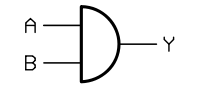
\includegraphics[width=0.3\textwidth]{200px-Logic-gate-and-de.png}
	\caption{Wikipedia \url{http://de.wikipedia.org/wiki/Logikgatter}}
	\label{und}
\end{figure}

\subsubsection{ODER}
\begin{figure}[ht]
	\centering
  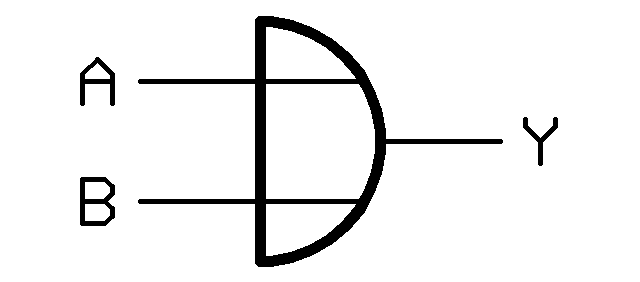
\includegraphics[width=0.3\textwidth]{Logic-gate-or-de.png}
	\caption{Wikipedia \url{http://de.wikipedia.org/wiki/Logikgatter}}
	\label{oder}
\end{figure}

\subsubsection{NICHT}
\begin{figure}[ht]
	\centering
  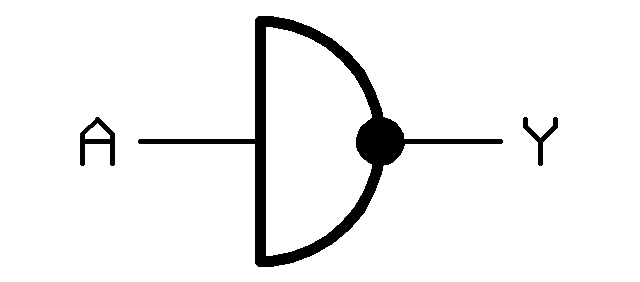
\includegraphics[width=0.3\textwidth]{Logic-gate-inv-de.png}
	\caption{Wikipedia \url{http://de.wikipedia.org/wiki/Logikgatter}}
	\label{nicht}
\end{figure}

\end{document}

